\chapter{Planning}
\label{chapter:planning}

This chapter covers the planning of the work and the task scheduling to be accomplished during the second semester to achieve the proposed objectives. The main tasks to be carried out are described below (the Gantt diagram in Fig.~\ref{fig:gantt} shows these activities displayed against time):

\begin{enumerate}
    \item \textbf{Overview of the Experimental Setup}. Familiarization with the robot and tools that will be used throughout the dissertation.

    \item \textbf{Development of Action Anticipation Models}. To formally define how to anticipate an action in the context of the collaborative task under study using RGB-D images as input. \acs{ml} models, such as \acfp{rnn}, are at the forefront of the algorithms to explore.
    
    \item \textbf{Development of an Anticipatory Controller}. To develop robot controllers that consider the human partner's movements and intentions and use these inferences to make appropriate decisions during the execution of a sequential assembly task.

    \item \textbf{Metrics and performance evaluation}. To provide performance metrics used to evaluate the action anticipation models and the add-value of the anticipatory controller (e.g., in terms of cycle time).
    
    \item \textbf{Thesis Writing}. Writing the master dissertation and other detailed documentation.
\end{enumerate}

\begin{sidewaysfigure}
\centering
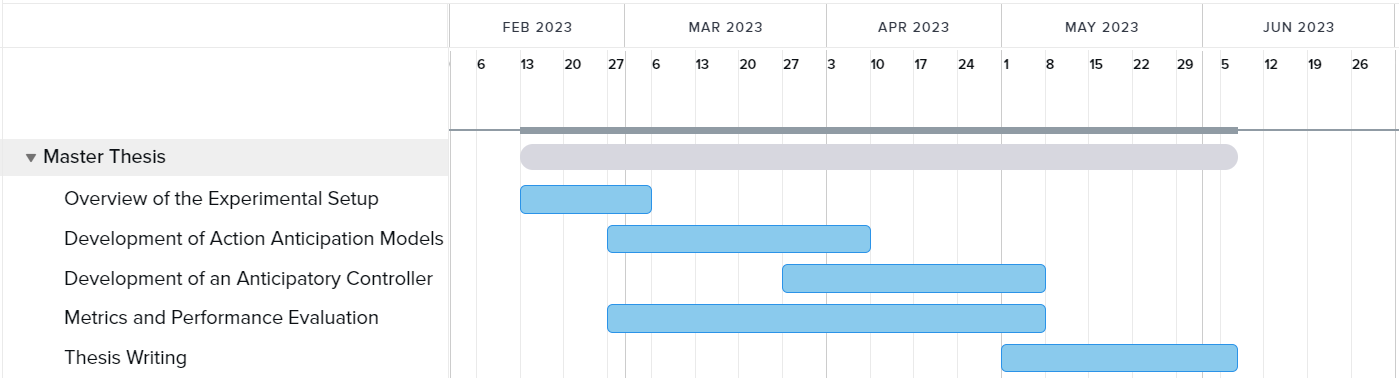
\includegraphics[width=9in]{figs/gantt.PNG}
\caption{Gantt Diagram of the Second Semester Tasks}
\label{fig:gantt}
\end{sidewaysfigure}
